\section{Proceduralne generowanie geometrii}
\label{sec:gen}
Reprezentacje opisane w rozdziale \ref{sec:rep} definiują jak geometria jest przechowywana i przetwarzana. Proceduralne generowanie dostarcza algorytmy, które tworzą lub zmieniają kształty według danych zasad. Pozwalają one na modyfikację bez ręcznego modelowania każdego szczegółu. Ten rozdział omawia dwa różne podejścia: powierzchnie subdywizyjne, które wygładzają istniejącą siatkę, oraz szumy, które generują dane od podstaw.

\subsection{Powierzchnie Subdywizyjne}
\label{sec:sub}
Powierzchnie subdywizyjne stanowią most między prostotą siatek o małej ilości wielokątów a gładkością powierzchni opartych na krzywych NURBS. Zamiast przetrzymywać duże ilości danych gęstej siatki, metoda przechowuję grubą siatkę bazową, która opisuje intencję kształtu a szczegóły produkuje proceduralnie.

\paragraph{Definicja i historia}
Siatki składające się z małej ilości wielokątów, nie pozwalają na skrupulatne odwzorowanie gładkich powierzchni. Chociażby krawędzie między ścianami są zawsze widoczne niezależnie od metody cieniowania. Powierzchnie subdywizyjne starają się rozwiązać ten problem poprzez zagęszczanie pierwotnej siatki iteracyjnie według zdefiniowanych zasad.

Edwin Catmull wynalazł metodę na generowanie powierzchni sześciennych dla dowolnych topologii. Natomiast nie był w stanie udowodnić, że powierzchnia jest stabilna w każdym punkcie, zdecydował się więc nie implementować jej. Jim clark wdrożył jego metodę i udowodnił empirycznie, że powierzchnia jest stabilna. W ten sposób pierwszym schematem, który powstał dla powierzchni czworokątnych był algorytm Catmull-Clark. Został on przedstawiony w 1978 roku jako uogólnienie rekursywnego podziału bikubicznych powierzchni B-splajnowych dla siatek o dowolnej topologii \cite{catmull1978}. Metoda jest zaprojektowana do produkowania powierzchni o ciągłości C2 wszędzie oprócz punktów nadzwyczajnych, w których spada do C1.

Schemat Loopa, został zaproponowany przez Charlesa Loopa w jego pracy magisterskiej z 1987 roku. Rozwiązuje on w niej ten sam problem co Catmull-Clark, lecz dla siatek trójkątnych \cite{warren2001, zorin2000}. Podobnie jak Catmull-Clark opiera się na uogólnieniu funckji B-splajnowych i produkuje powierzchnie z ciągłością C2 wszędzie poza punktami nadzwyczajnymi, gdzie wynosi C1.

Wierzchołek nadzwyczajny jest takim, który ma walencję, czyli liczbę przylegających krawędzi do wierzchołka, inną niż cztery. W standardowych sekcjach siatki, powierzchnia graniczna jest powierzchnią B-splajnową \cite{catmull1978, hughes2013}.

\paragraph{Zasada działania}
Algorytm Catmull-Clark działa na siatce czworokątów i iteracyjnie wprowadza trzy rodzaje nowych wierzchołków. Punkt ściany $\mathbf{f}$ to średnia wszystkich wierzchołków, które definiują daną ścianę. Punkt krawędzi $\mathbf{e}$ jest średnią dwóch krańców danej krawędzi oraz dwóch punktów ścian, które sąsiadują z daną krawędzią. Nową pozycję istniejącego wierzchołka $\mathbf{v}$ wyznacza się przez:
\begin{equation}
    \mathbf{v}' = \frac{\mathbf{Q}}{n} + \frac{2\mathbf{R}}{n} 
    + \frac{(n-3)\mathbf{S}}{n}
\end{equation}
gdzie $n$ to walencja, $\mathbf{Q}$ to średnia nowych punktów ścian które przylegają do wierzchołka, $\mathbf{R}$ to średnia punktów środkowych przylegających krawędzi, i $\mathbf{S}$ jest starą pozycją wierzchołka \cite{catmull1978}.

Po obliczeniu wierzchołków, siatka jest modyfikowana przez połączenie punktów ścian z punktami krawędzi oraz punktów krawędzi z nowymi wierzchołkami. Każdy czworokąt jest podzielony na cztery mniejsze, co sprawia że każda iteracja zwiększa ilość ścian czterokrotnie.

\begin{figure}[h!]
    \centering
    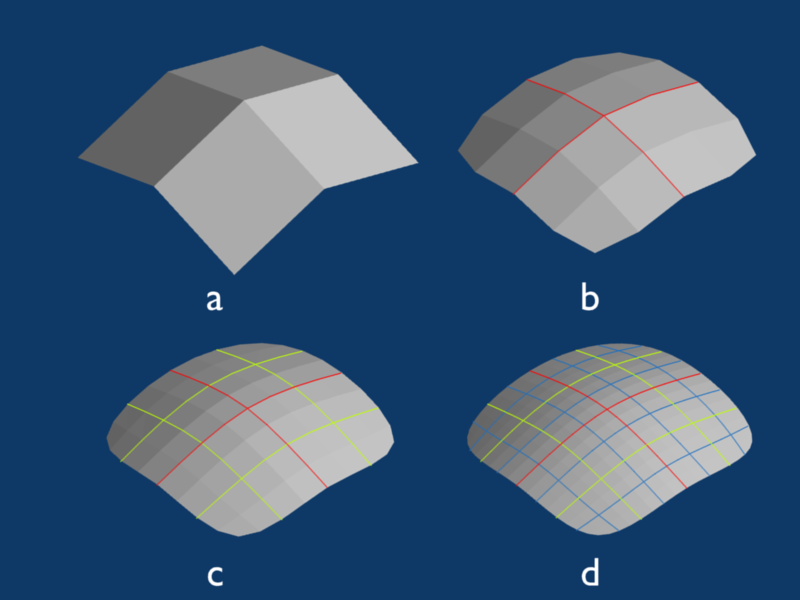
\includegraphics[width=0.8\columnwidth]{media/Catmull-Clark.png}
    \caption{Wizualizacja podziału algorytmem Catmull-Clark. Banlu Kemiyatorn, via Wikimedia Commons}
    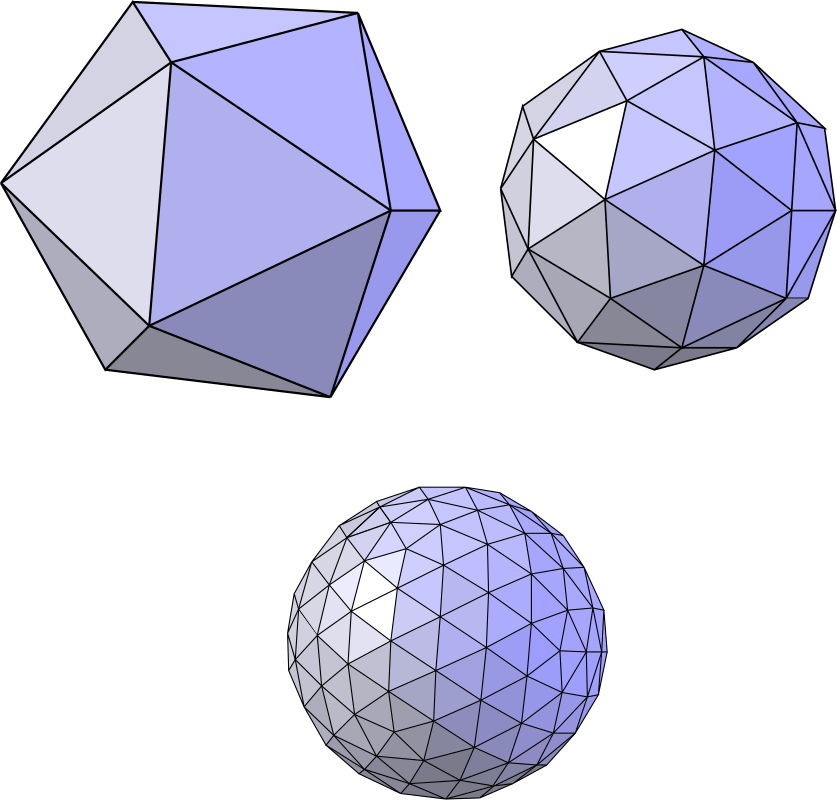
\includegraphics[width=0.8\columnwidth]{media/Loop.png}
    \caption{Wizualizacja podziału algorytmem Loopa. Simon Fuhrmann, CC BY-SA 3.0, via Wikimedia Commons}
    \label{fig:catmull}
\end{figure}

\paragraph{Warianty}
Schematy można podzielić na aproksymujące i interpolacyjne, kategoryzacja zależy od tego czy wierzchołki siatki bazowej są zachowane w powierzchni granicznej. W modelach aproksymujących, takich jak Catmull-Clark i Loop, wierzchołki są przesuwane w każdej iteracji, a punkty kontrolne nie leżą na powierzchni granicznej, natomiast są one jej przybliżeniem. W schematach interpolacyjnych, takich jak Modified Butterfly i Kobbelt \cite{warren2001}, wierzchołki siatki bazowej nie są modyfikowane i powierzchnia graniczna dokładnie przechodzi przez punkty kontrolne.

Interpolacja pozwala na bezpośrednią kontrolę punktów, które leżą na końcowej powierzchni, co upraszcza obliczenia. Niestety natomiast jakość powierzchni interpolacyjnych jest niższa niż aproksymujących, zbiegają wolniej do granicy i są bardziej podatne na artefakty \cite{zorin2000}.


\paragraph{Zastosowania}
Powierzchnie podziału są rozlegle wykorzystywane w animacji filmowej. Pixar wprowadził je do produkcji przy \textit{Geri's Game} (1997), a dwa lata później wydali artykuł w którym opisali szczegóły \cite{derose1998}. Główną motywacją był problem z deformacją, animowane postacie wymagają gładkich powierzchni przy zginaniu stawów. W tym wypadku gęste siatki wprowadzają artefakty na krawędziach. Podział siatki z niską ilością wielokątów rozwiązuje ten problem.

Programy do modelowania trójwymiarowego takie jak Blender czy Maya, wykorzystują algorytm Catmull-Clark jako standardowy modyfikator do użytku. Artysta może modelować siatkę o niskiej rozdzielczości a podział jest zastosowany przy renderowaniu. W grach komputerowych zastosowanie jest rzadsze przez koszt obliczeniowy w czasie rzeczywistym.

\paragraph{Zalety i wady}
Jedną z głównych zalet powierzchni subdywizyjnych jest kompaktowość reprezentacji, złożone topologie mogą być opisane siatkami z małą ilością wierzchołków. Inną zaletą jest gładkość powierzchni granicznej, która jest zagwarantowana matematycznie oraz fakt, że edycja siatki jest intuicyjna, ponieważ artysta może kontrolować bezpośrednio punkty kontrolne.

Ograniczeniem tej metody jest trudność w kontrolowaniu ostrych krawędzi, ponieważ algorytm polega na wygładzaniu geometrii co wymusza wykorzystywanie dodatkowych technik. Kolejną wadą jest koszt obliczeniowy, który wraz z liczbą iteracji rośnie wykładniczo. Dodatkowo punkty nadzwyczajne wprowadzają artefakty przez zaburzenie ciągłości w ich otoczeniu \cite{catmull1978}.

\subsection{Szumy Proceduralne}
Szum Perlina i inne szumy proceduralne rozwiązują inny problem niż powierzchnie subdywizyjne, zamiast modyfikować geometrię która już istnieje, generują dane bez ręcznego modelowania. Są one fundamentalną techniką w każdym miejscu gdzie jest potrzeba na kontrolowaną losowość.

\paragraph{Definicja i historia}
Ken Perlin opracował funkcję szumu pracując nad efektami wizualnymi do filmu \textit{TRON} (1982) w \textit{Information International Inc}. Celem było stworzenie tekstur proceduralnych, które wyglądają organicznie. Dotychczasowe metody opierały się na białym sumie, który nie ma żadnej koherencji przestrzennej i jest całkowicie losowy. W papierze \cite{perlin1985} z 1985 Perlin opisuje system teksturowania, którego szum jest częścią. Za swój algorytm Perlin dostał w 1997 nagrodę w Akademii Filmowej, co ukazuje jak dramatyczną zmianą było przedstawienie tej metody. W 2002 Perlin opublikował nowy artykuł \cite{perlin2002} w którym opisał poprawy, które wprowadził do swojego oryginalnego algorytmu, eliminując dwa ograniczenia z poprzedniej metody.

Steven Worley w 1996 roku zaproponował inne podejście do szumu proceduralnego \cite{worley1996}. Zamiast interpolować gradient na siatce, wartość funkcji zależy od odległości do najbliższego z losowo położonych punktów. Produkuje to wzory, które w kształcie przypominają organiczne struktury takie jak kamień lub skóra. W przeciwieństwie do szumu Perlina, który charakteryzuje się gładkimi przejściami.

\paragraph{Zasada działania}
Szum Perlina jest definiowany dla punktu $\mathbf{x} = (x, y, z)$ trzema krokami. Pierwszy to przypisanie pseudo-losowego wektora gradientu do każdego wierzchołka w siatce liczb całkowitych, które otaczają dany punkt. Gradienty są wyznaczone na podstawie wcześniej obliczonych tablicy permutacji $P$ i gradientów $G$. Tablica $P$ haszuje wierzchołki siatki do indeksu tablicy $G$, co pomimo pozornej losowości jest deterministyczne.

Kolejnym krokiem jest wyznaczenie iloczynu skalarnego między wektorem gradientu wierzchołka a wektorem odległości od tego wierzchołka do punktu $\mathbf{x}$. Następnie interpoluje się trójliniowo osiem takich wartości za pomocą funkcji:
\begin{equation}
    s(t) = 3t^2 - 2t^3
\end{equation}
Oryginalny algorytm posiada dwie wady. Pierwszą z nich jest niezerowa druga pochodna funkcji $s(t)$ dla $t=0$ i $t=1$, co wytwarza artefakty przy cieniowaniu. Drugą jest faworyzacja niektórych kierunków nad innymi spowodowana doborem gradientów \cite{perlin2002}.

Szum Worleya działa na innej zasadzie, wykorzystuje losowe rozrzucenie punktów $\mathbf{c}_i$, gdzie wartość funkcji jest wyznaczana przez odległość do najbliższego punktu:
\begin{equation}
    w(\mathbf{x}) = \min \|\mathbf{x} - \mathbf{c}_i\|
\end{equation}
Dzięki kombinacją odległości od pierwszego, drugiego oraz trzeciego najbliższego punktu, można otrzymać różne wizualnie szumy \cite{worley1996}.

\begin{figure}[h!]
    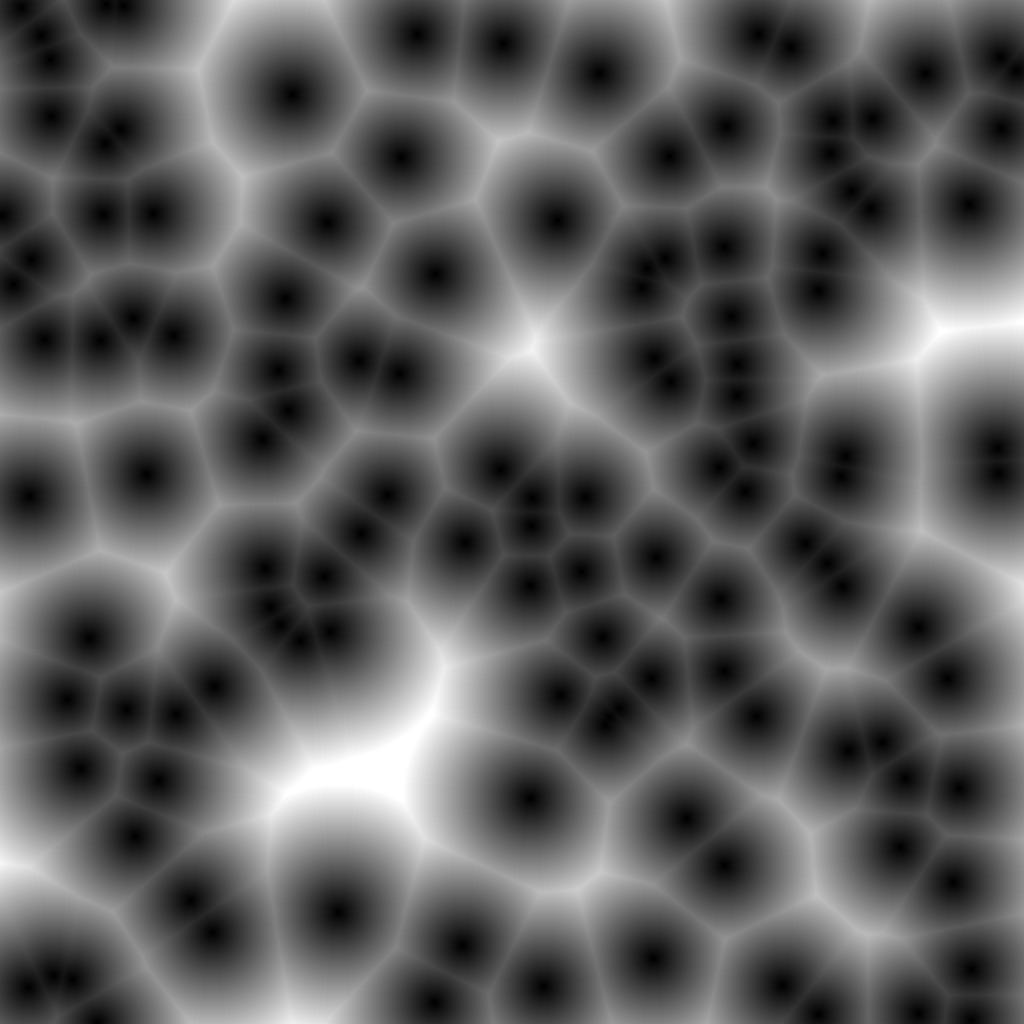
\includegraphics[width=\columnwidth]{media/Worley.jpg}
    \caption{Wizualizacja szumu Worleya. Rocchini, CC BY-SA 3.0, via Wikimedia Commons}
    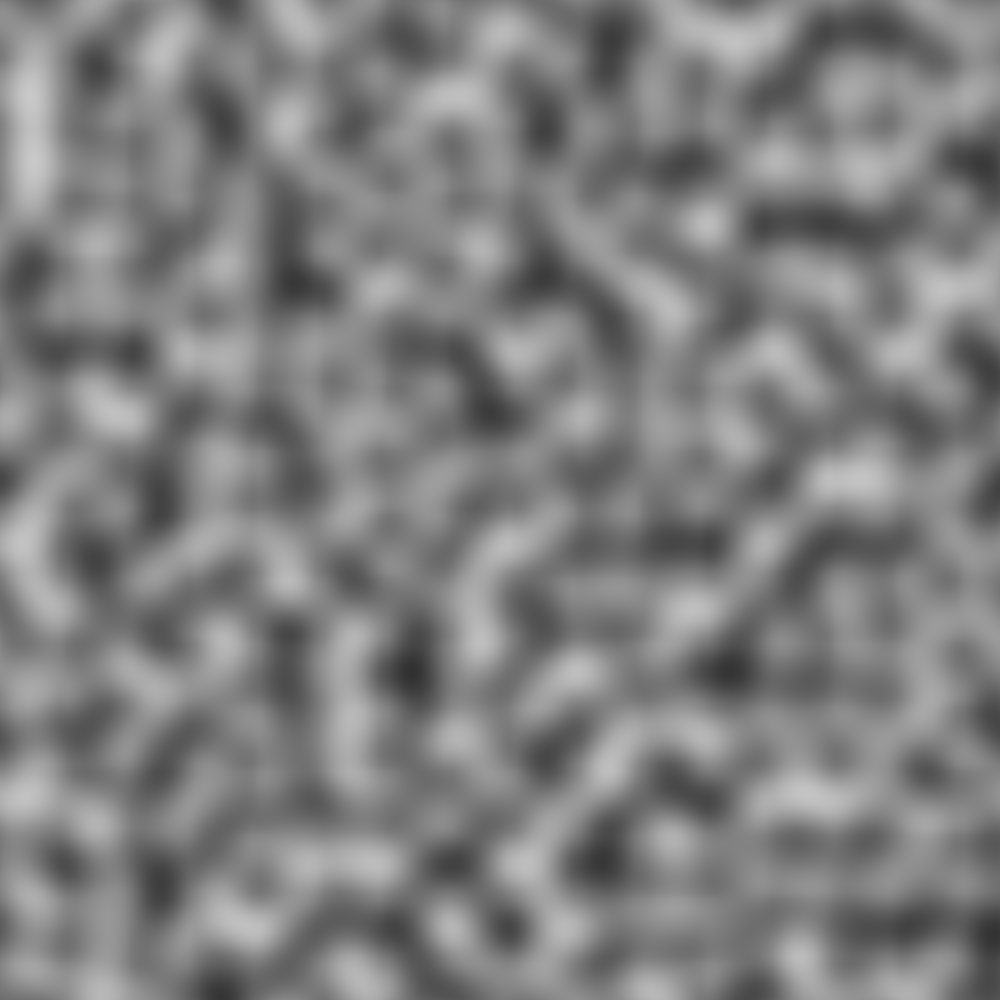
\includegraphics[width=\columnwidth]{media/Perlin.png}
    \caption{Wizualizacja szumu Perlina. Lord Belbury, CC0, via Wikimedia Commons}
\end{figure}

\paragraph{Warianty i rozszerzenia}
W swojej pracy z 2002 roku, Perlin opisał poprawiony algorytm szumu. Jedną z dwóch zmian którą wprowadził względem oryginału było zamienienie funkcji wygładzającej na:
\begin{equation}
    s(t) = 6t^5 - 15t^4 + 10t^3
\end{equation}
zapewnia ona ciągłość C2, czyli pierwsza i druga pochodna jest zerowa dla $t=0$ i $t=1$, dzięki czemu wyeliminowano artefakty cieniowania. Kolejną zmianą której dokonał Perlin było zastąpienie możliwych gradientów z pełni losowych na ograniczony zbiór, dzięki czemu pozbył się faworyzowania kierunków. Pomimo tych zmian algorytm wciąż jest około 10\% szybszy \cite{perlin2002}.

\textit{Simplex noise}, zaproponowany przez Perlina w \cite{perlin2001}, zastępuje siatkę sześcienną, siatką simpleksową. W trzech wymiarach simpleks jest czworościanem. Koszt obliczeniowy siatki sześciennej w $n$ wymiarach wymaga $2^n$ wierzchołków. W przeciwieństwie do tego siatka simpleksowa redukuje tą złożoność do $n+1$ wierzchołków, co dla trzech wymiarów zmniejsza osiem do czterech wymaganych wierzchołków.

\paragraph{Zastosowania}
Najbardziej znanym zastosowaniem szumu Perlina jest proceduralne generowanie terenu. Wartości szumu są próbkowane i tworzą mapę wysokości, która jest później przekształcana w siatkę trójkątną.

Innym kluczowym zastosowaniem są tekstury proceduralne. Wykorzystanie szumu Perlina pozwala na generowanie tekstur które imitują drewno, chmury czy ogień, więc wzory które wynikają naturalnie z przekształcenia szumu, a ciężko odwzorować ręcznie. Z kolei szum Worleya wykorzystuje się do teksturowania chociażby kamienia lub skóry.


\paragraph{Zalety i wady}
Główną zaletą szumów proceduralnych jest determinizm, gdzie ta sama wartość ziarna zawsze zwróci identyczny wynik, dzięki czemu można wykorzystywać generowane dane bez potrzeby przechowywania ich. W przeciwieństwie do szumu białego, szum Perlina posiada ciągłość przestrzenną co jest jego fundamentem. Drugą ważną zaletą jest niski i stały koszt obliczeniowy dla pojedynczego punktu.

Natomiast głównym ograniczeniem tych metod jest widoczna regularność przy niskich częstotliwościach, co ujawnia się jako powtarzająca struktura. Szum Perlina nie nadaje się do reprezentacji ostrych krawędzi, jako że wytwarza tylko gładkie i organicznie wyglądające przejścia. Mniejszą, ale znaczącą wadą jest kontrola, parametry pozwalają na ustalenie ogólnego charakteru wygenerowanych danych, ale nie pozwalają na sterowanie szczegółami.